
A seqencial data is highly complex and difficult to understand. Once the sequence data is collected, we have to convert the data into a meaningful representation. Information in log files can be analyzed by building operational profiles \cite{hmf08}\cite{nwv09}. In operational profiling, we determine how many times each subset of events occurs in the sequence data. Serial ordering of events in a sequence data is very unintuitive to perform any analyses. In an editor, we can view maybe 60-70 lines at any one point. However, many times,we need to go through thousands of lines in the sequence data to arrive at some meningful information due to repeating patterns. Hence, it is difficult to compare events that are separated by other events. For example if a specific sequence of 4 events occurs 5\% of the times in a log file with 500,000 events, then that is 25,000 (5\% of 500,000) events that we have to analyze to make any conclusion. In addition, the remaining events will be in between these repeating patterns.

we can analyse the data accurately and efficiently by transforming the serially ordered events in a sequence data to a Weighted Directed Graph (WDG) data structure. Only the information needed for the analysis need to be maintained and condensed into a compact view of the log file. We can abstract the information in the log line to any level, such as, event level, method level, class level, file level, sub-module level, or module level.

                \begin{enumerate}
                \item Convert sequence data to usage data :
In the sequence data, each event is important as a standalone event. However, in the WDG representation, the importance shifts to adjacent pairs of events. We do this type of a transformation to record the order in which events happened. Therefore, each unique event in the sequence data is represented by a unique node in the WDG. An edge exists from one node (head) to another (tail) if there is an occurrence of the event representing the tail node immediately after the event representing the head node in the original log file. For example if event B follows event A in the log file, then there is directed edge from node A to node B in the WDG. The edges are labeled with the number of times this transition has occurred.  For example if B occurs a fifty times after A in the log file, then the edge from node A to node B in the WDG is labeled with 50. Typically, we keep track of the actual count as the weight of the edge, when building the graph. 
\begin{figure}[!t]
\centering
\includegraphics[width=4in]{Graphics/op-profile-example.png}
\caption{Weighted Directed Graph of the Example Log File}
\label{WDG_example}
\end{figure}

In the graph we display the percentage value as the label. This percentage is propotional to the total number of transitions.  The cumulative probability of out-edges of a node is 1. The transitional probabilities of each out-edges are calculated by dividing the number of transactions of that out-edge with the sum of all outward transactions from that node. We could also store the dynamic parameter information in each log line as a list along the edges. We now present the steps involved in this transformation. Consider that the input log file is with $N$ log lines. We need to convert this log file WDG.
\begin{enumerate}
\item First pass through the $N$ lines of the log file: Parse the log message in each log line of the log file as static event information (or event identifier) and dynamic parameter information \cite{mnv10}. Assign an identifier (ID) to each unique event (defined by the static information in the log message in that log line) in the log file. Simultaneously create and update an index file with the (ID, event) pairs as new ones are detected in the log file. Let the number of indexes in total be $M$.
\item Create the adjacency matrix $G$, an $M*M$ matrix. Each entry in the matrix represents the number of transitions between the events corresponding to the particular row and column. However, we could store more information in the matrix if we choose to, like the dynamic parameter information. 
\item Second pass through the $N$ lines of the log file: If $i$ is the current line that we are inspecting, then find the event ID in line $i$ and $i+1$. Then retrieve the current count at $G[eventID(i)][eventID(i+1)]$. Increment the integer.
\item Once the entire log file has been transformed into the adjacency matrix, we can render the graph using tools like Graphviz \cite{gviz} or ORA \cite{ora}.  Alternately, we could apply analysis algorithms, like the ones explained in detail in Section \ref{analyses}, on the adjacency matrix $G$, and highlight the results when the graph is rendered.
\end{enumerate}

The complexity of this transformation is linear in the size of the log file, i.e. $O(N)$, where $N$ is the number of lines in the log file. Step 1 makes a single pass through the log file, and examines each log line. Hence, the time complexity of step 1 is $O(N)$. In step 1, we inspect each line of the log file. For each line, we do an array access in the two-dimensional adjacency matrix $G[M][M]$. Since array access takes constant time, this step too is $O(N)$. Step 6 iterates through each element of the adjacency matrix $G[M][M]$. Thus, it is of the order $O(M^2)$. Since\[ M << N\$, \$M^2 < N \] Hence the order of time complexity for the transformation is $O(N)$, or linear in the size of the log file. The two data structures we create from the log file with N log lines is the index of size $O(M)$, and the adjacency matrix $G[M][M]$ of size $O(M^2)$. Since $M^2 < N$, the space occupied by the output is much smaller than the input log file.

To explain the steps with an example, consider a simple log file where the activities are spearated by commas. $1-2, 2-3, 3-4, 4-5, 5-4, 4-5, 5-4, 4-6, 6-7, 7-5, 5-4, 4-5, 5-4, 4-5, 5-8, 8-9$. The events in the log file are mapped to their corresponding event IDs: $1, 2, 3, 4, 5, 4, 5, 4, 6, 7, 5, 4, 5, 4, 5, 8, 9$. Each node is a unique event. An edge between nodes 1 and 2 signifies that the event 2  appears after event 1  in the log file. The labels on the edges have the actual count and could have the transitional probabilities as well. The transitional probability from node 1 to node 2 is 1.0, whereas the transitional probability from node 4 to node 6 is 0.2. The adjacency matrix representation of the example WDG is in table \ref{Adjacency_example_log}. This is depicted in Fig \ref{WDG_example}.

\begin{table}[!t]
%\renewcommand{\arraystretch}{1.3}
\caption{Adjacency Matrix Representation of Example Log File}
\label{Adjacency_example_log}
\centering
\begin{tabular}{|c|c|c|c|c|c|c|c|c|c|}
\hline
  {\bf ID} &    {\bf 1} &    {\bf 2} &    {\bf 3} &    {\bf 4} &    {\bf 5} &    {\bf 6} &    {\bf 7} &    {\bf 8} &    {\bf 9} \\
\hline
   {\bf 1} &          0 &          1 &          0 &          0 &          0 &          0 &          0 &          0 &          0 \\
\hline
   {\bf 2} &          0 &          0 &          1 &          0 &          0 &          0 &          0 &          0 &          0 \\
\hline
   {\bf 3} &          0 &          0 &          0 &          1 &          0 &          0 &          0 &          0 &          0 \\
\hline
   {\bf 4} &          0 &          0 &          0 &          0 &          4 &          1 &          0 &          0 &          0 \\
\hline
   {\bf 5} &          0 &          0 &          0 &          4 &          0 &          0 &          0 &          1 &          0 \\
\hline
   {\bf 6} &          0 &          0 &          0 &          0 &          0 &          0 &          1 &          0 &          0 \\
\hline
   {\bf 7} &          0 &          0 &          0 &          0 &          1 &          0 &          0 &          0 &          0 \\
\hline
   {\bf 8} &          0 &          0 &          0 &          0 &          0 &          0 &          0 &          0 &          1 \\
\hline
   {\bf 9} &          0 &          0 &          0 &          0 &          0 &          0 &          0 &          0 &          0 \\
\hline
\end{tabular}  
\end{table} 

Operational profiling involves determining which sequences of actions are repeating across the log. Using our adjacency matrix representation of the log file, we can determine the operational profile of the system. 

JUMBL (Java Usage Model Builder Library) developed by Software Quality Research Laboratory (SQRL) of University of Tennessee \cite{jumbl} can be used for developing operational profile and calculating the probability of usage by each state of the operational profile. JUMBL is a collection of tools to support automated, model-based, statistical testing of systems \cite{jug}. JUMBL helps in

\begin{itemize}
\item Constructing usage models from component states
\item Generating tests in various ways
\item Converting tests to executable data to support test automation, and
\item Assessing testing by providing test measures, including expected system reliability in the field.
\end{itemize}

WDG along with the transitional probability are used to determine the state probabilities of each component . We have used JUMBL to create the state probabilities \cite{anil}. We have converted the WDG to JUMBL readable TML \cite{tug} language. As described in Section \ref{transform}, we have developed tools, which will mine the log file and convert the log file to an adjacency matrix representation with the number of transitions from each node, which is translated directly to TML script. A sample log file is and the corresponding TML fileare given below. The TML script has information about the nodes, the out edges from each node along with the number of transitions from each node to another. This TML script is used in JUMBL to arrive at the state probabilities of each node. State probabilities give information about the percentage of usage of each node. Corresponding graph is depicted in Fig. \ref{fig:op-profile-example}



\begin{alltt}
\small{ \emph{
2013-03-21 18:18:32Z,A
2013-03-21 18:18:33Z,B
2013-03-21 18:20:49Z,C
2013-03-21 18:20:50Z,A
2013-03-21 18:20:56Z,B
2013-03-21 18:20:57Z,A
2013-03-21 18:21:08Z,C
2013-03-21 18:21:08Z,D
2013-03-21 18:21:08Z,E
2013-03-21 18:21:08Z,A
}}
\end{alltt}

\begin{alltt}
\small{ \emph{

// Usebased model for testlog

($ fill(1) $)
model testlog
//use this before each transition to show probability ($0.10$)

source [A]
($2$)"Count=2 (A->B), TimeElapsed= 7secs" [B]
($1$)"Count=1 (A->C), TimeElapsed= 11secs" [C]

[B]
($1$)"Count=1 (B->C), TimeElapsed= 136secs" [C]
($1$)"Count=1 (B->A), TimeElapsed= 1secs" [A]

[C]
($1$)"Count=1 (C->A), TimeElapsed= 1secs" [A]
($1$)"Count=1 (C->D)" [D]

[D]
($1$)"Count=1 (D->E)" [E]

[E]
($1$)"Count=1 (E->A)" [A]


"exit" [Exit]

end 
}}
\end{alltt}


\begin{figure}
  \centering
  \includegraphics[scale=.58]{../Graphics/op-profile-example.png}
  \caption{WDG example}\label{fig:../Graphics/op-profile-example.png}
\end{figure}


A sequence data with hundreds of thousands of lines can be quickly convereted to more meaningful graphical represeantation using this method. Once the TML file is generated, we can use JUMBL to find out the state probabilities of each states. usaing the state probaility and the usage patterns we can arrive conclusions and can visualize them easily like mentioned in figures  \ref{sample_log} and \ref{fig:log_with_color}

\begin{figure}
  \centering
  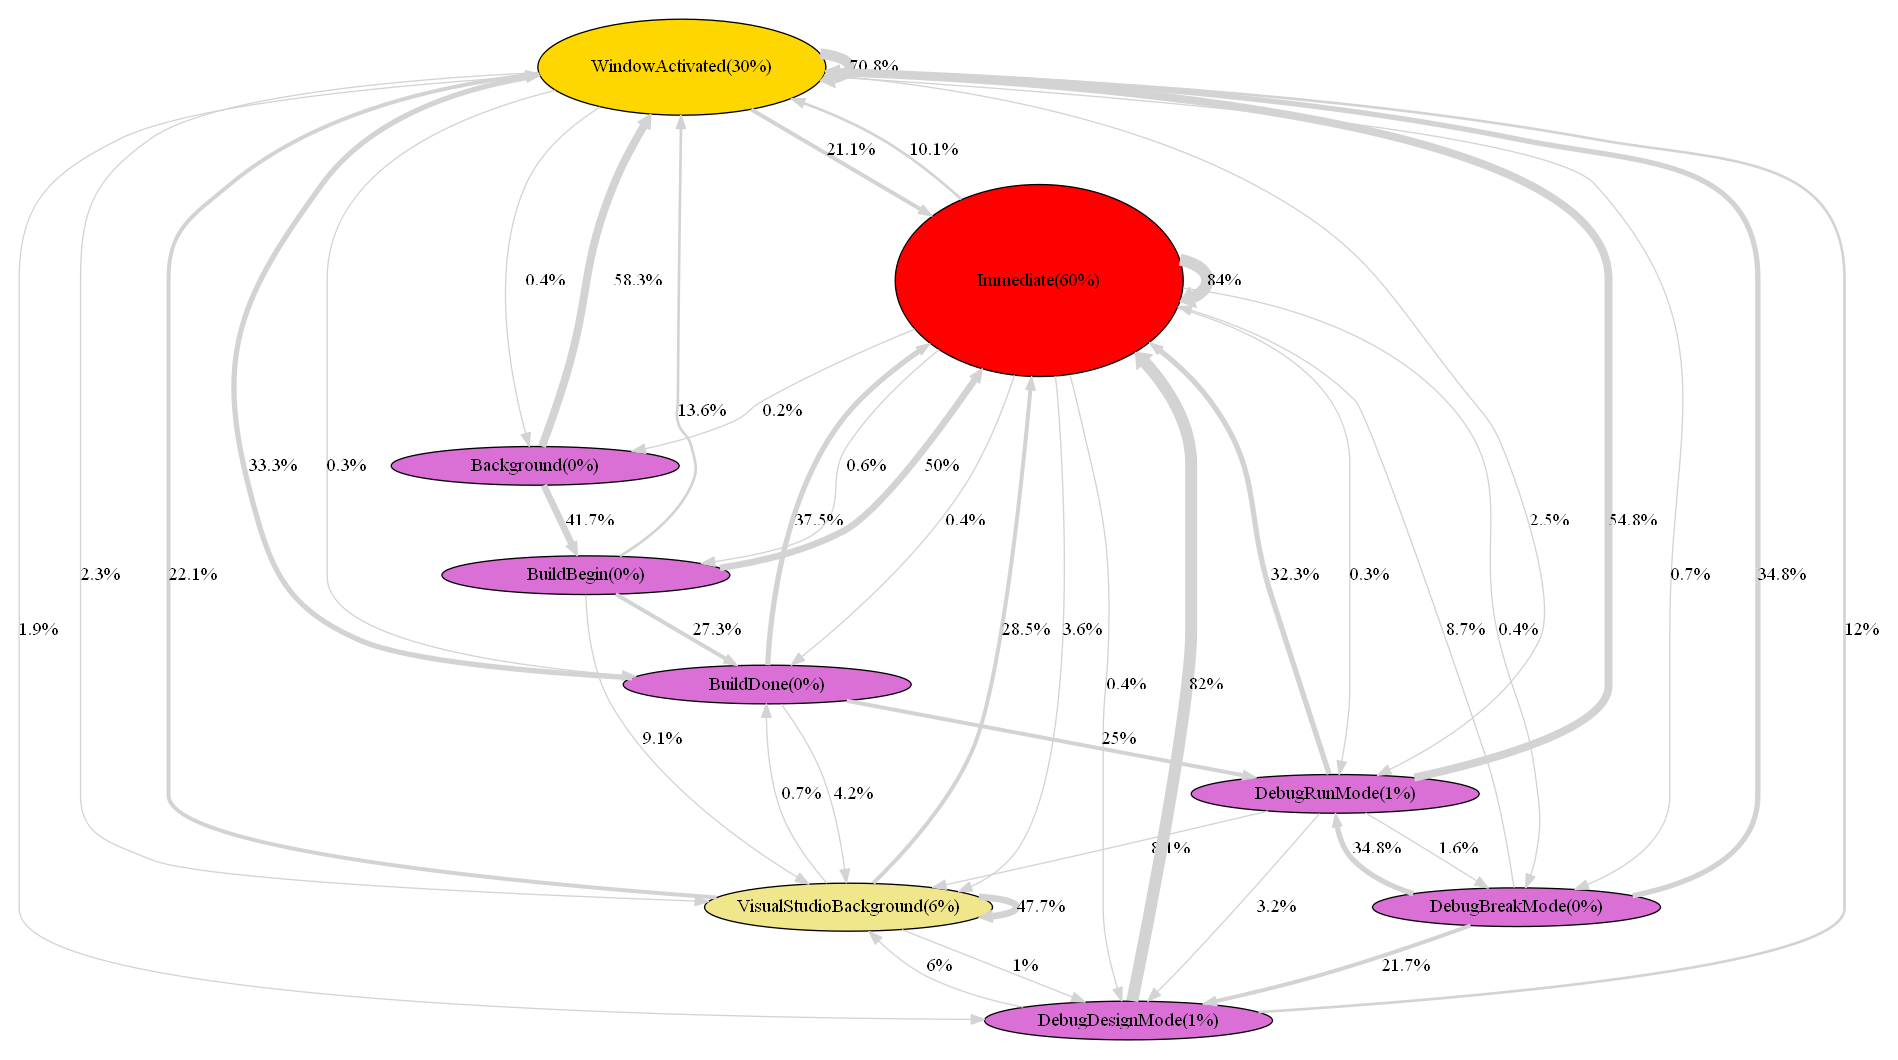
\includegraphics[scale=.20]{../Graphics/log_with_color.png}
  \caption{WDG example with probaility}\label{fig:log_with_color}
\end{figure}

\begin{figure}
  \centering
  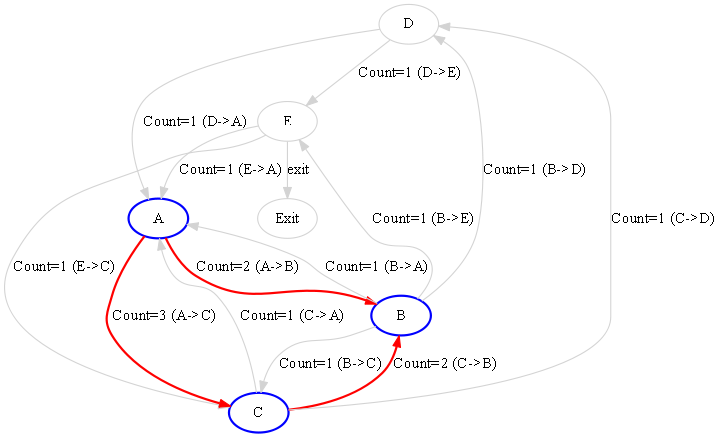
\includegraphics[scale=.58]{../Graphics/sample_log.png}
  \caption{WDG example with probaility}\label{fig:sample_log}
\end{figure}

                
	\end{enumerate}


